\chapter{Development}
The goal of this chapter is to illustrate the new implementations and changes to the project's software, describing the improvements of the previous features, the new ones and the way in which they have been achieved.
\bigbreak

In the previous project's code, some time and memory optimizations have been made, minor bugs have been found and fixed and some other improvements have been done (e.g. replacing deprecated methods and libraries with newer ones).

\section{MQTT QoS2 caching}
As mentioned in the \textit{Unsolved Issues} chapter of Dario Piotrowicz's thesis \cite{Pio19}, there was a problem with unreliable Wi-Fi networks (an issue in the library's GitHub repository is still open \cite{githubQos2Issue}): all messages generated while a broken client-broker connection were discarded, instead of being stored to be sent when the connection will be re-established.

To solve that issue have been implemented two caching queues, one for each connection: the playing session one and the neural network's pattern collection one.

The cache size has been set to a safe value of 32 kilobytes (tested experimentally: bigger values led the Photon out of memory more often than not). The maximum number of messages that can be cached is stored in the \texttt{cache\_size} variable. With a maximum message size of 512 characters (511 effective characters because of the null terminator), the value is easily calculated as 32.

The following is a graph of the playing session's connection caching implementation; the neural network one is analogous.
\bigbreak

\begin{lstlisting}[style=CPPStyle]

	...

	// ready to send the data (publishString) to the client
	if (client.isConnected()) {
        while (cached_messages.size() > 0) {
			// send cached messages
            std::string msg = cached_messages.front();
            cached_messages.pop();
			client.publish("motiontracker/" + ID,
							msg.c_str(),
							MQTT::QOS2);
        }
		client.publish("motiontracker/" + ID,
						publishString,
						MQTT::QOS2);
    } else if (cached_messages.size() < cache_bound) {
		// save message in cache
        std::string msg(publishString);
        cached_messages.push(msg);
    }

	...

\end{lstlisting}
\bigbreak

This solution has made possible to damper temporary disconnections caused by instable connections.

\section{Delay in real-time data plotting}
\dots

\section{Motion capture}
In the software's previous version, developed and improved by Dario Piotrowicz \cite{Pio19} from the Marco Lanini's project \cite{Lan17}, the data processed by the device and sent to the server were:
\begin{itemize}
	\item device's orientation both in quaternions and yaw, pitch and roll angles;
	\item device's acceleration in Cartesian and spherical coordinates system;
	\item raw accelerometer, gyroscope and magnetometer data;
	\item device's velocity approximation.
\end{itemize}

This work's aim is to detect \textit{discriminating features among different playing patterns}, by collecting and analyzing the sensors data stream; the analysis followed the flow in the data fusion schema (Figure \ref{old data fusion schema}), except for the velocity approximation.
\bigbreak

The velocity approximation, calculated by the \textit{Velocimeter} class \cite{Pio19}, was early excluded because of the practical difficulty in obtaining realistic values using only inertial sensors, where measurement errors are unavoidable, especially for miniature MEMS sensors \cite{Du15, Est14, Kow15, Liu01, Sei07, UsingAcc, Woo07, Yan06}.

Direct integration of acceleration often causes unrealistic drifts in velocity, due to errors propagation; furthermore, measured acceleration not only carries random noise, but also presents with offset caused by temperature drift \cite{Kow15, Liu01, Woo07}, resulting in estimation errors accumulated by integration process, that results in low accuracy.

In particular, two behaviors were miscalculated:
\begin{itemize}
	\item stillness after a movement: if the truck toy is pushed from behind and it is left to stop alone, the velocity is expected to linearly decrease down to zero, but the velocity graph shows an uniform-like decrease in the first phase, and a peak towards zero in the last one;
	\item repetitive light accelerations: the vertical acceleration generated by the tessellated tyres rolling resulted in absent vertical velocities.
\end{itemize}

\begin{center}
	\begin{figure}[ht]
		\makebox[\textwidth]{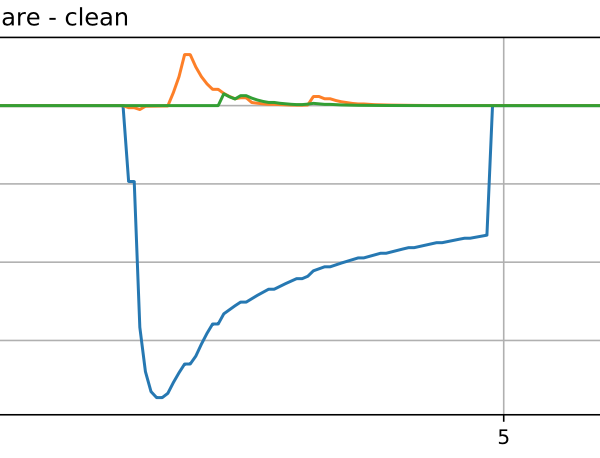
\includegraphics[width=0.2\paperwidth]{img/plots/square.png}}
		\caption{Square wave and absent velocities.}
	\end{figure}
\end{center}

\subsection{Gravity-affected data}
The first analytic phase dealt with raw accelerometer data, but the signal's noisiness and the presence of gravity have induced to desist. Nevertheless, especially for movements with strong accelerations, that simply increase the signal-to-noise ratio, the main waveform was recognizable.
\bigbreak

TODO: graph
\bigbreak

The analysis moved to Kalman-filtered data, which proved to be much cleaner and smoother, but still influenced by gravity; thus it would have been necessary a more complex training data collection, due to the lack of orientation invariance – the gravity decomposes among the axes in accordance with device's orientation, influences other accelerations, and affects the neural network's training: the neural network would believe that the gravity is part of the pattern acceleration; consequently, the same pattern recorded with a different device's orientation would be classified differently. To achieve such invariance it would be necessary to collect every pattern with the device rotated in any possible angle.
\bigbreak

TODO: graph
\bigbreak

Nevertheless, it was discovered that the gravity-free acceleration computed by the device and sent to the server was not stored in the database, but only used for the 3D visual representation. It was decided to store such data in the database along with other sensors data, and analyze it to see whether it was reliable over time. A smooth gravity-free acceleration could have been the turning point for an efficient neural network training and future classification.
\bigbreak

\subsection{Gravity-free data}
Analyzing gravity-free data, another problem showed up: after a few minutes of playing, the calculation of the yaw angle accumulated errors that led it to diverge in an unrealistic way, rotating counterclockwise, and consequently the accelerations no longer matched the device's orientation. The error didn't grow with the still device, but only when the device was moved, and therefore it should not be confused with the \textit{yaw drift} problem, that leads the yaw to rotate constantly in any device condition, and it's often caused by biases in gyroscope measurements (and that's the case of this project \cite{Pio19}) or poor/absent magnetometer calibration.
\bigbreak

The yaw's measurement was particularly affected by rotations around the Earth's $z$-axis (in other words, over the plane generated by the $x$ and $y$ axes), and the bigger the pitch angle, the bigger the error, as shown in the table below. Pitch and roll, on the contrary, were calculated almost without errors.
\bigbreak

\begin{table}[ht]
	\centering
	\begin{tabular}{c|c c}
	\textbf{Pitch} ($^{\circ}$) & \textbf{Mean error} ($^{\circ}$) & \textbf{Standard deviation} ($^{\circ}$) \\ \hline
	0                           & 47.12                            & 0.94                                     \\
	20                          & 47.67                            & 1.88                                     \\
	40                          & 51.14                            & 1.45                                     \\
	60                          & 58.14                            & 1.73                                     \\
	80                          & 57.80                            & 0.75
	\end{tabular}
	\caption{Yaw errors after a 360$^{\circ}$ rotation with different pitch angles.}
\end{table}

\begin{center}
	\begin{figure}[ht]
		\makebox[\textwidth]{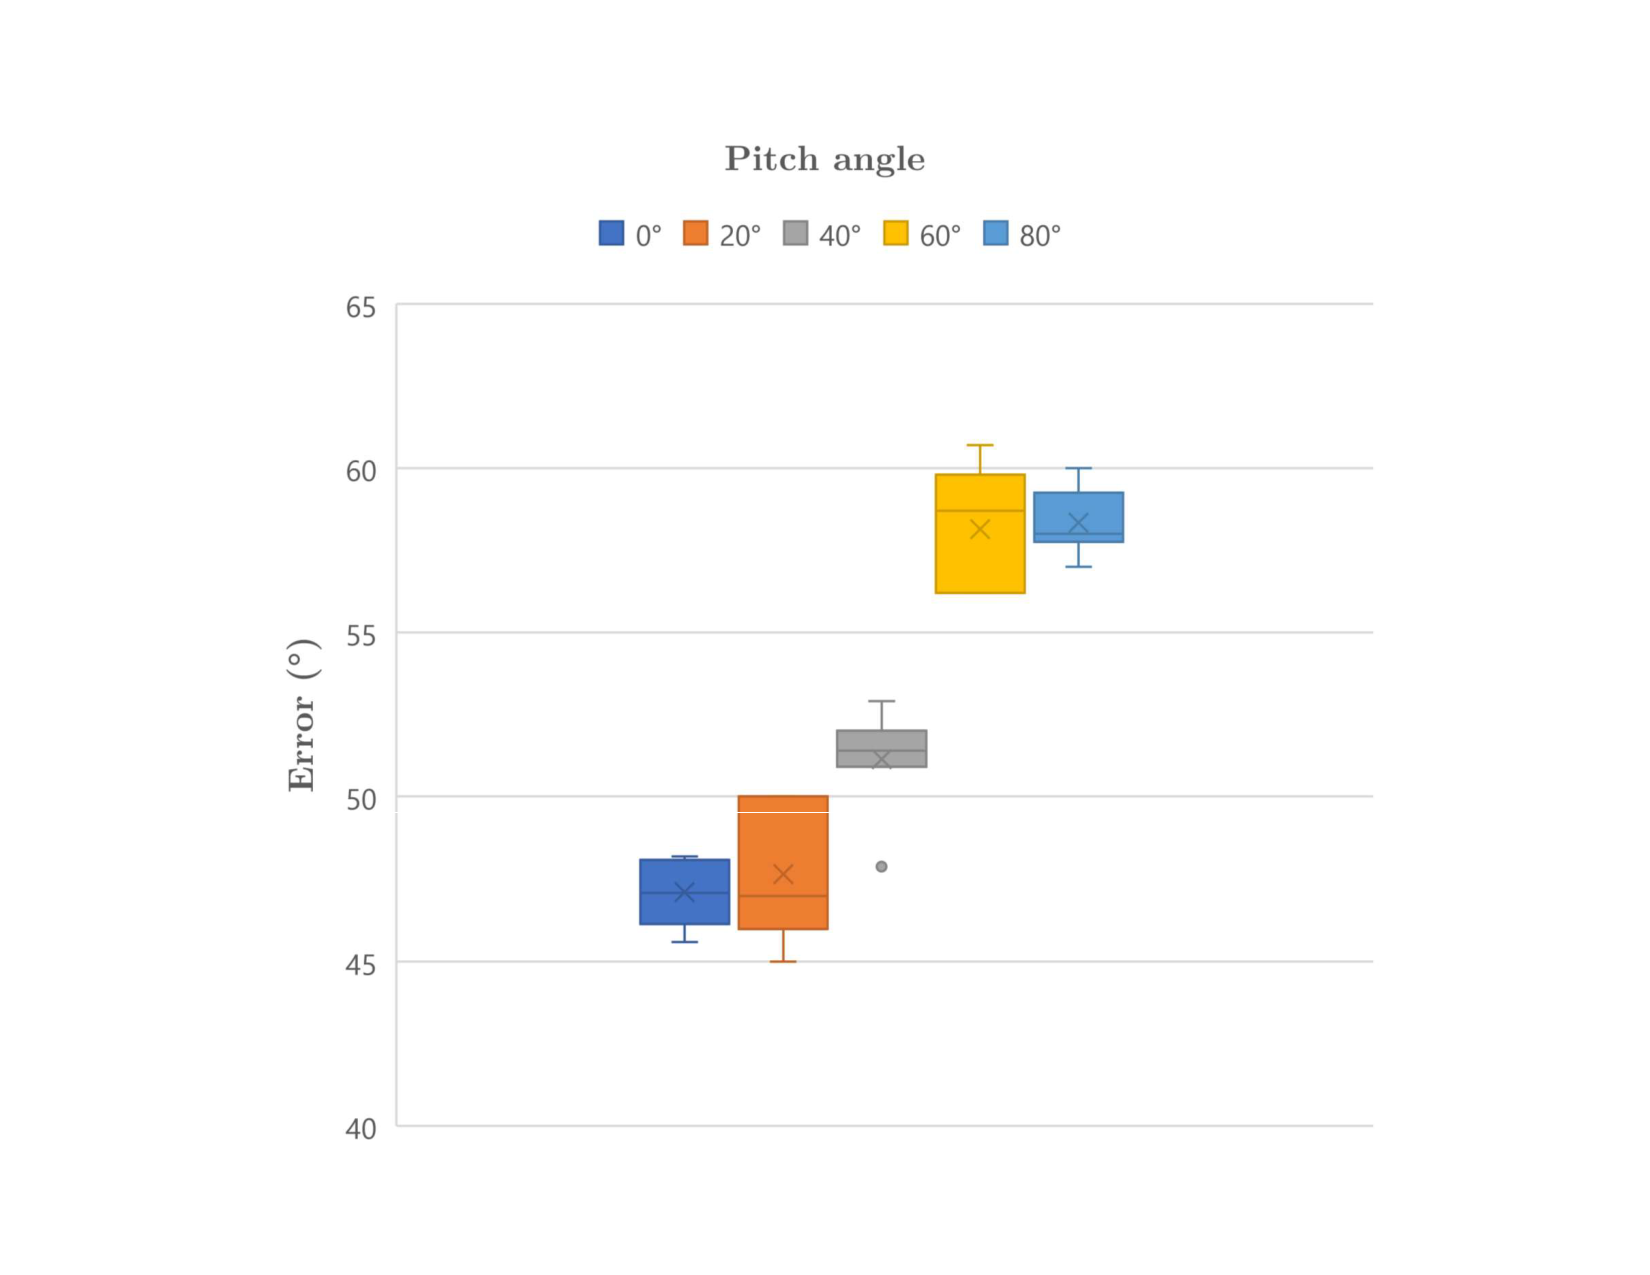
\includegraphics[width=0.55\paperwidth]{img/yaw_errors.pdf}}
		\caption{Box plot of yaw errors.}
	\end{figure}
\end{center}

Small yaw variations were also noticed with pitch-only movements: after a 360$^{\circ}$ rotation, the mean error was 0.47$^{\circ}$ with a standard deviation of 0.11$^{\circ}$.

\begin{center}
	\begin{figure}[ht]
		\makebox[\textwidth]{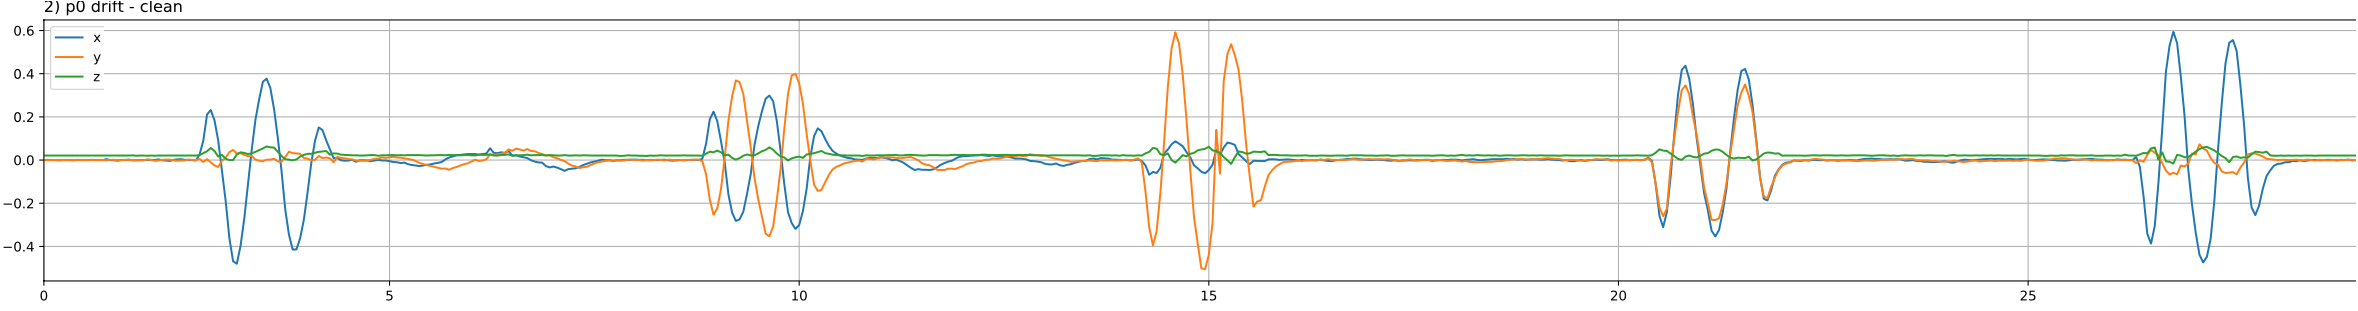
\includegraphics[width=0.7\paperwidth]{img/plots/drift.png}}
		\caption{Different accelerations for the same pattern.}
	\end{figure}
\end{center}

During some tests, it was noticed another unexpected behavior: different recordings of the same pattern with different device rotations showed the same acceleration among axes (e.g. given a fixed three-dimensional path, following it with the truck facing forwards, backward, upside-down or other, would show exactly the same accelerations).
\bigbreak

TODO: Plot with the same movement with different orientations that shows the same data
\bigbreak

The cause of the error was discovered to be in the Madgwick's algorithm implementation, more precisely in the lack of yaw's convergence in its error-correction gradient descent phase (see section \ref{Madgwick filter}). Unfortunately, several algorithm implementations that included the correction, and different values of the algorithm's gain parameter (the magnitude $\beta$ of the gyroscope measurement error\footnote{Increasing $\beta$ leads to faster bias corrections and higher sensitiveness to lateral accelerations.} \cite[13]{Mad10}) gave no better results over time, and worse, ghost accelerations were found. Then, the Lanini's version has been kept and the troubleshooting continued.
\bigbreak

Since the accelerations were independent from the orientation of the device, the cause was necessarily the reference system's location, which proved to be global: the movements were shown as viewed by an external observer, placed in the Earth's center.

To align the reference system back, it was sufficient to rotate the acceleration vector by the 3 orientation angles (of \textit{yaw}, \textit{pitch} and \textit{roll}) given by the Madgwick's algorithm, and that, as shown below, not only correctly brought the reference system back to a local point of view, but surprisingly solved the yaw alignment issue.

The explanation of this (apparent) side-effect lies in how the gravity subtraction is performed: as shown in the Figure \ref{old data fusion schema}, the data obtained from the Kalman and Madgwick filters are used jointly. As discussed above, the Kalman filter does not present any problem, while the Madgwick one fails in the yaw angle calculation; hence, the resulting acceleration is misaligned, and needs to be corrected by the same misalignment angle: the Madgwick's angle itself.
\bigbreak

The rotation of the acceleration vector has been performed through a three-dimensional rotation matrix. In three-dimensional matrices, the matrix-vector multiplication doesn't affect the speed meaningfully, even for relatively weak CPUs like the one that runs in the Photon: the goal packets' frequency of 22 Hertz \cite{Pio19} has been always achieved (when the wireless connection allowed it) and however the C++ code is compiled by \texttt{GCC} with the \texttt{-Os} flag, that includes the loop unrolling optimization \cite{UsingGCC}.

\begin{center}
	\begin{figure}[ht]
		\makebox[\textwidth]{
\includegraphics[width=0.7\paperwidth]{img/plots/nodrift.png}}
		\caption{Image of correct accelerations.}
	\end{figure}
\end{center}

\subsection{Fine tuning: magnetic distortions}
Once achieved a reliable gravity-filtered acceleration approximation, it was possible to perform some fine tuning.
\bigbreak

It is known that magnetic and inertial sensors can be influenced by magnetic disturbance \cite{Fan17}.
There are two types of magnetic distortions:
\begin{enumerate}
	\item \textit{soft iron}: it's a temporary influence that appears when a material is affected by the Earth's magnetic field, and it's induced from metals that are non permanently magnetised (they don't generate a magnetic field themselves) \cite{Cro15}. It causes errors in the measured direction of the Earth's magnetic field, and since it depends on the orientation of the material relative to the sensor and the magnetic field, it cannot be compensated by a constant \cite{CompensatingIron};
	\item \textit{hard iron}: it's produced by materials that exhibit a constant, additive field to the Earth's magnetic field \cite{CompensatingIron}, and it can be simply removed by a constant offset, calculated through calibration \cite{CompensatingIron, Geb06, Kok12}.
\end{enumerate}

Madgwick's algorithm is able to remove \textit{soft iron} distortions \cite[11-12]{Mad10}, and the calibration to remove \textit{hard iron} distortions has been performed by the SparkFun's Arduino library.
\bigbreak

Unfortunately, there are non-constant interferences that still affect the sensors readings, such as the magnetic field generated by the current passing through the USB cable for charging the battery.
Its removal is much harder, because requires to analyze how much current is flowing through the cable, and the knowledge of the net magnetic field's shape, that depends on how the cable is placed around the sensor.

\begin{center}
	\begin{figure}[ht]
		\makebox[\textwidth]{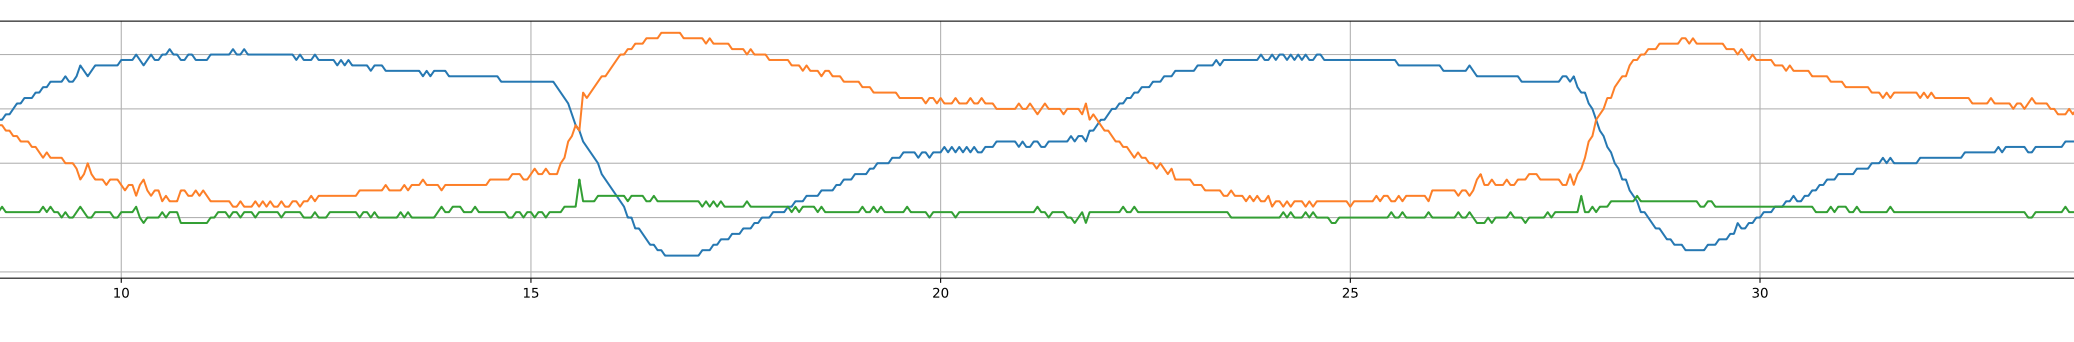
\includegraphics[width=0.7\paperwidth]{img/plots/battery.png}}
		\caption{Orientation affected by the battery charging.}
	\end{figure}
\end{center}

\subsection{Final data fusion schema}
The current data flow is illustrated by the schema:

\begin{center}
	\begin{figure}[ht]
		\makebox[\textwidth]{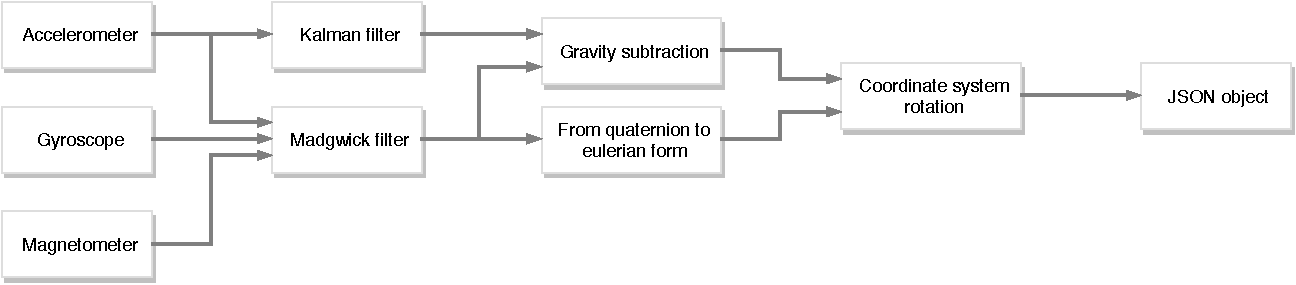
\includegraphics[width=0.65\paperwidth]{img/data_fusion.pdf}}
		\caption{Current data fusion schema.}
	\end{figure}
\end{center}

\subsection{Smart pattern recording}
Previously, the recording of a pattern for the training set was simply triggered by specific buttons in the web page, that once pressed, started immediately the recording. Since the recording time was quite short (500ms), it was difficult to start moving the toy exactly when the server started recording, because the movement could start too early or too late: both can cause data loss, but the second case is subtly more dangerous, including movements unrelated to the pattern inside the recording.

To prevent unintended movements from being saved, the recording module was modified in this way: the buttons no more trigger the immediate start of the recording, but sends the server in a \textit{waiting} state, an intermediate state where it asynchronously waits the toy to being moved. When the toy is moved, the real recording starts, without any data loss.

The motion detection is performed by the toy itself, and sent to the server through an attribute in the JSON object; unfortunately it has been found a slight delay between the real movement and its detection, empirically measured as 150ms, that corresponds to 3 packets, sent by the device but discarded by the server: to solve this problem, a small buffer has been included within the recording module, and these packets are punt in front of the ones that would be saved before.

\begin{center}
	\begin{figure}[ht]
		\makebox[\textwidth]{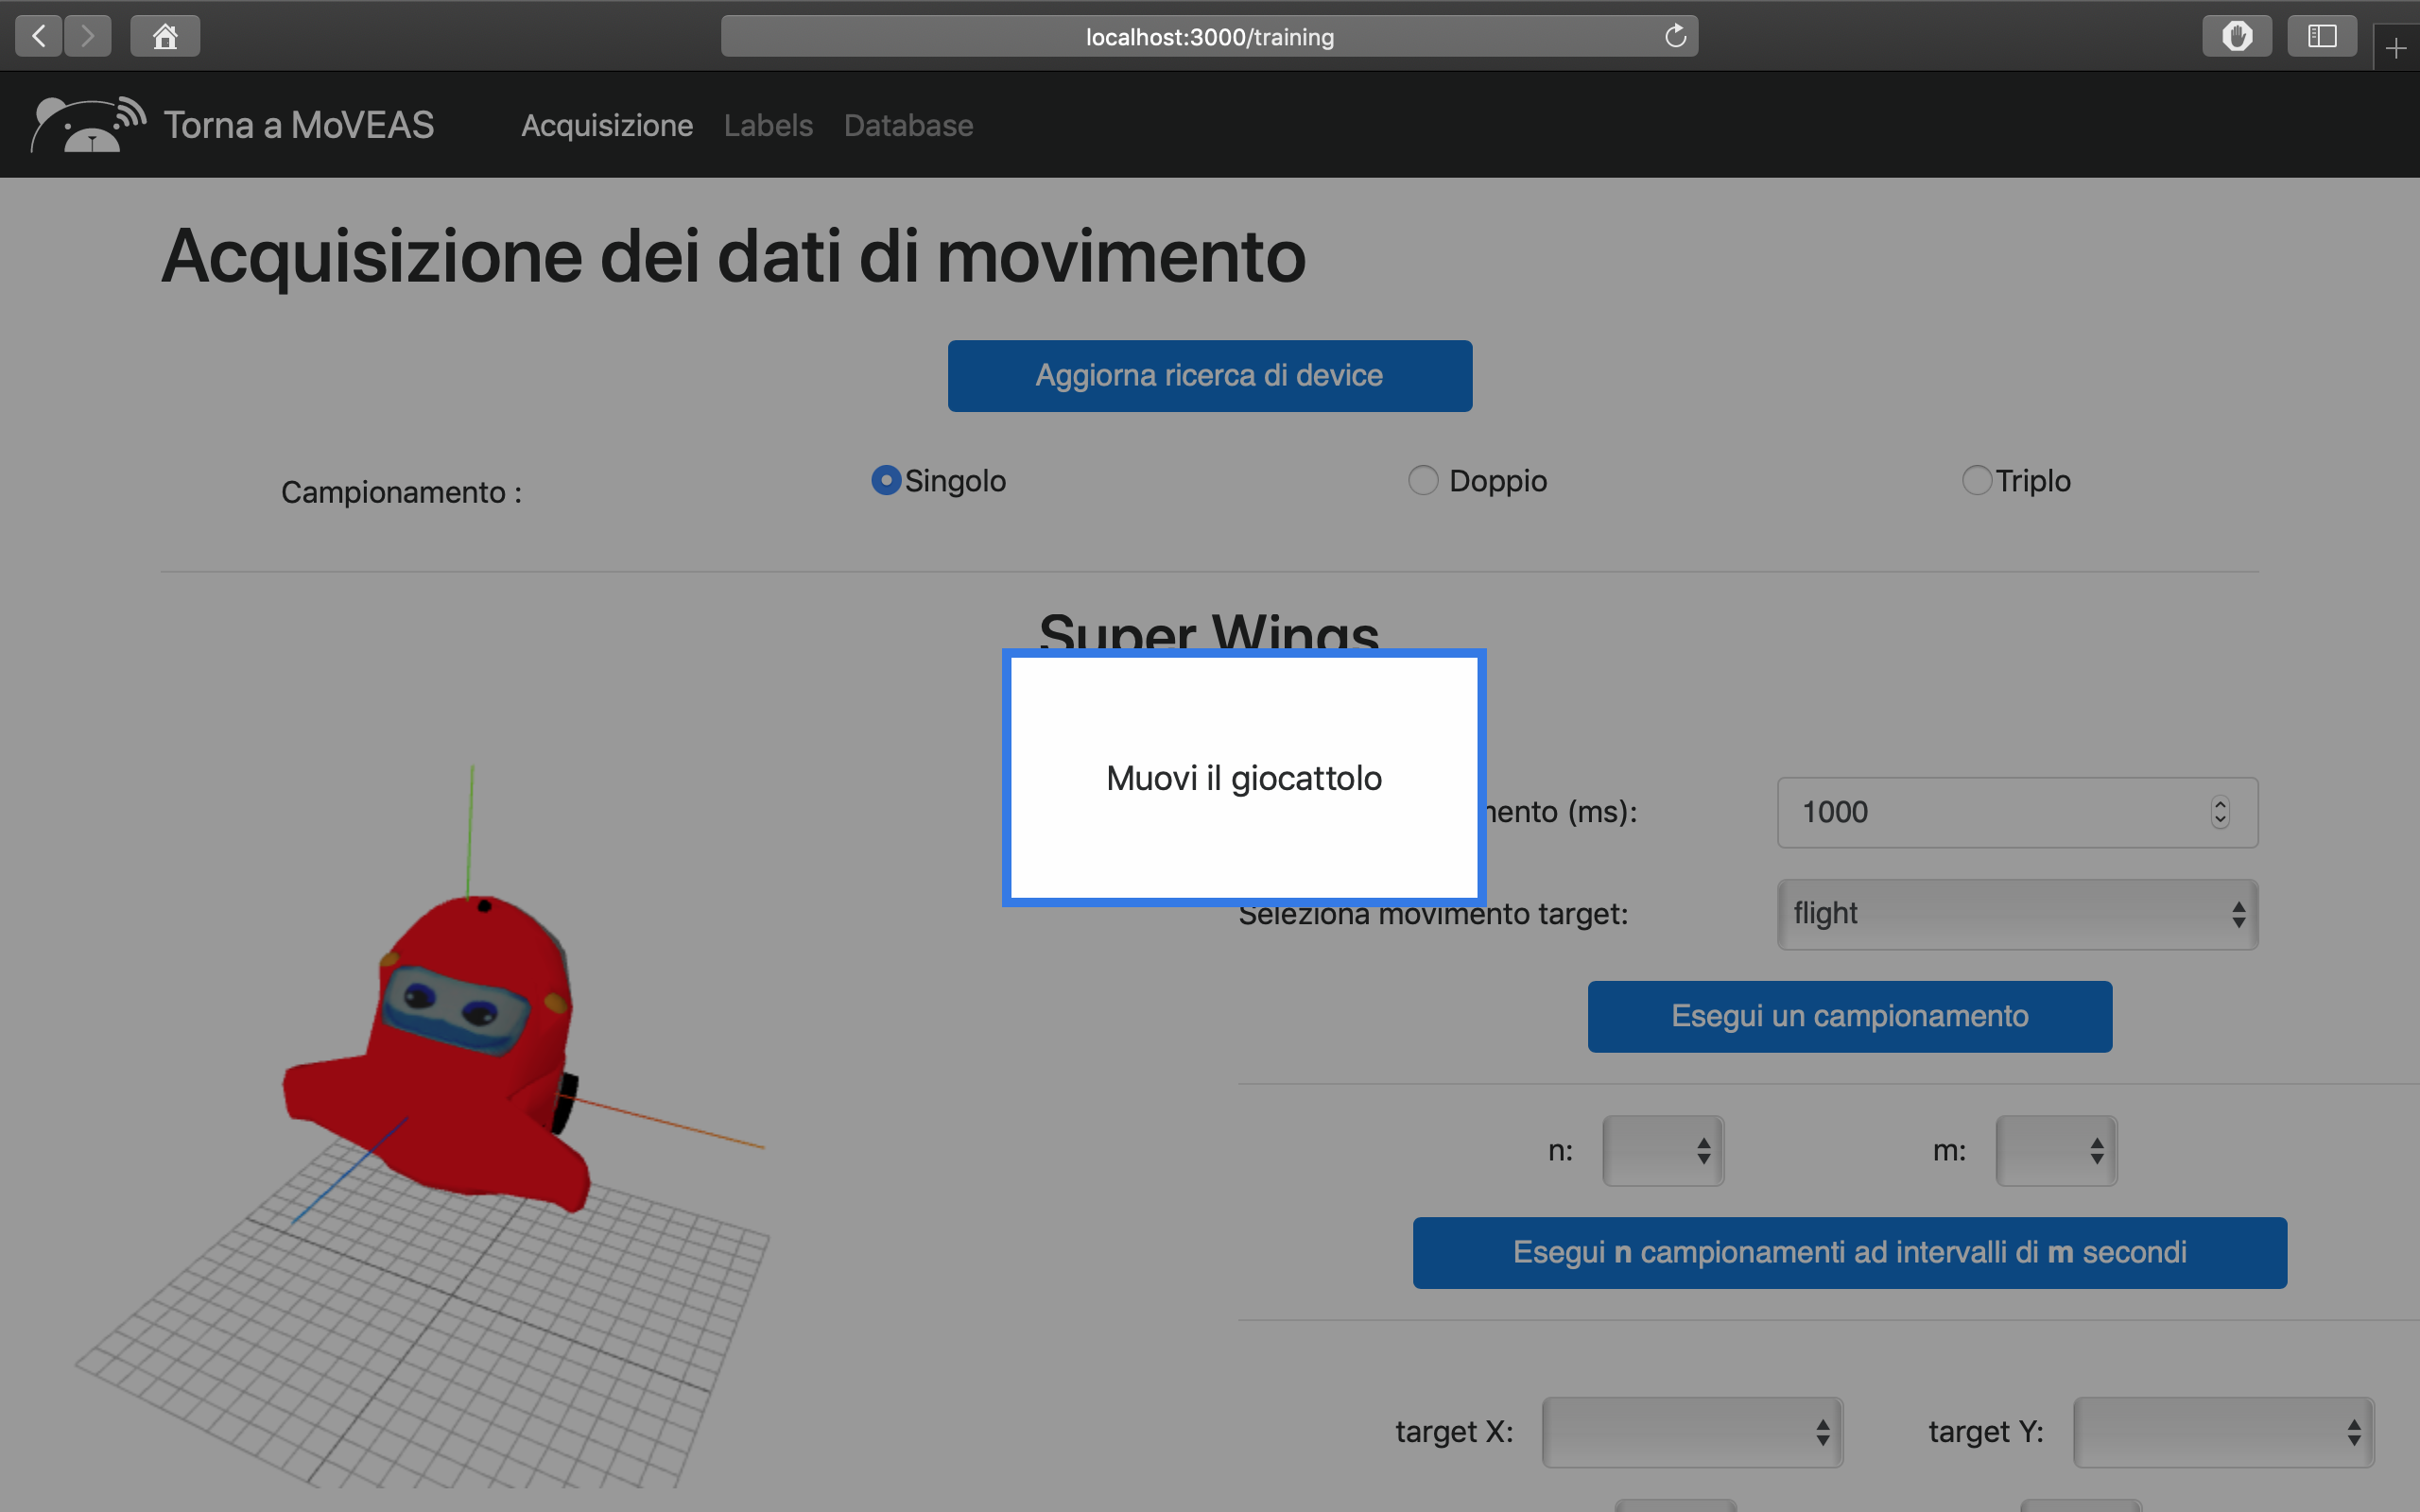
\includegraphics[width=0.6\paperwidth]{img/wait.png}}
		\caption{The recording module the waiting state.}
	\end{figure}
\end{center}
Not all patterns need the same recording time: for example, the movement of the toy pushed forward is much smaller than the one where the toy is thrown against a pillow, where the toy is thrown by the hand first, then flies in the air until it reaches the pillow. To adapt the module to this eventuality, it has been added the possibility to change the duration of the recording. Nevertheless, not every neural network can deal with variable-length sequences.

\section{Time series classification}
Standard feedforward neural networks are not suitable for time series classification tasks, because they are not \textit{shift-invariant} (in this case, time-invariant). For time series patterns, this allows the network to classify a pattern regardless of its start time.

\subsection{Dataset}
For model training and validation, the dataset was composed of:
\begin{itemize}
	\item 100 patterns with the toy going \textit{forward} and 100 with the toy going \textit{backward};
	\item 200 patterns of simulated \textit{flight};
	\item 200 patterns with the \textit{still} toy;
	\item 200 patterns of the toy carried while \textit{walking};
	\item 200 patterns of the toy \textit{thrown} against a pillow.
\end{itemize}
The training and validation portions were respectively the 60\% and the 40\% of the total, and the entire dataset is shuffled before every training.

The test set was composed of 240 samples, disjoint from the training and validation ones.
\bigbreak

In this work, two network's models have been chosen, and their performance compared. The first one is a time delay neural network, chosen for its simplicity, since the training sequences were short (22 samples) and a complex model might go very easily to overfitting; the second one is a recurrent neural network, chosen for its ability to recognize variable-length patterns.

The following part explains how the model selection was done.
\bigbreak

\subsection{Time delay neural network}
\subsubsection{Topology and activation functions}
The model selection started from the simplest topology: an input layer with data normalization, a convolutional hidden layer with a \textit{ReLU} activation function, that performed better than \textit{tanh}, and an output layer for the pattern classification, with a \textit{softmax} function, to obtain values between 0 and 1, representing the probability of the classified pattern to belong to each possible class.
\bigbreak

\begin{center}
	\begin{figure}[ht]
		\makebox[\textwidth]{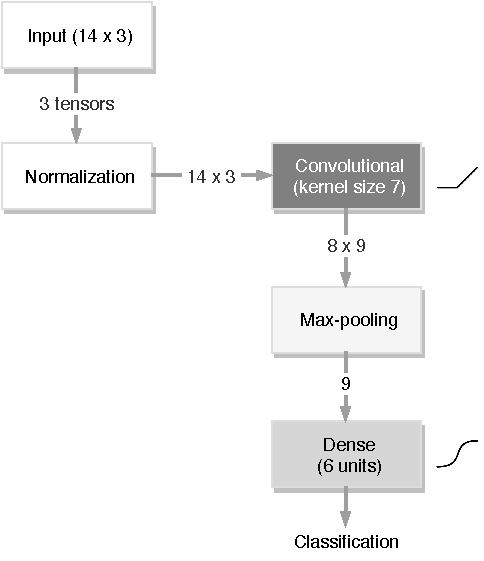
\includegraphics[width=0.35\paperwidth]{img/tdnn_topology.pdf}}
		\caption{TDNN final topology.}
	\end{figure}
\end{center}

\subsubsection{Features}
Only three features were considered relevant for the training: the gravity-free accelerations values in the three axes. Some tests showed quickly that adding more features, like orientation, velocity data, or raw sensors data, made the network almost untrainable with this simple model.

\subsubsection{Hyperparameters}
The search for the two most important hyperparameters, the \textit{kernel} size and the number of \textit{filters}, has been performed through a \textit{grid search}. For each table's entry, the network has been tested 10 times, with shuffled data between testing and validation set for each run. Outliers have been omitted from the average.

\begin{table}[ht]
	\centering
	\begin{tabular}{cccccc}
									  &                         & \multicolumn{4}{c}{\textbf{Kernel size}} \\
									  & \multicolumn{1}{c|}{}   & 3        & 5        & 7        & 9       \\ \cline{2-6} 
	\multirow{7}{*}{\textbf{Filters}} & \multicolumn{1}{c|}{3}  & 90,00\%  & 92,57\%  & 95,00\%  & 98,25\% \\
									  & \multicolumn{1}{c|}{5}  & 94,50\%  & 95,50\%  & 98,50\%  & 99,00\% \\
									  & \multicolumn{1}{c|}{7}  & 98,80\%  & 99,00\%  & 99,87\%  & 99,90\% \\
									  & \multicolumn{1}{c|}{9}  & 97,93\%  & 99,00\%  & 99,65\%  & 99,87\% \\
									  & \multicolumn{1}{c|}{11} & 98,06\%  & 98,52\%  & 99,59\%  & 99,83\% \\
									  & \multicolumn{1}{c|}{13} & 96,94\%  & 99,53\%  & 99,91\%  & 99,84\% \\
									  & \multicolumn{1}{c|}{15} & 99,20\%  & 99,88\%  & 99,90\%  & 99,90\%
	\end{tabular}
	\caption{Average training accuracy.}
\end{table}

\begin{table}[ht]
	\centering
	\begin{tabular}{cccccc}
									  &                         & \multicolumn{4}{c}{\textbf{Kernel size}}       \\
									  & \multicolumn{1}{c|}{}   & 3       & 5       & 7            & 9           \\ \cline{2-6} 
	\multirow{7}{*}{\textbf{Filters}} & \multicolumn{1}{c|}{3}  & 77,68\% & 81,50\% & 92,33\%      & 87,33\%     \\
								      & \multicolumn{1}{c|}{5}  & 87,17\% & 92,73\% & 95,25\%      & 94,53\%     \\
									  & \multicolumn{1}{c|}{7}  & 90,38\% & 97,92\% & 95,68\%      & 95,25\%     \\
									  & \multicolumn{1}{c|}{9}  & 95,50\% & 97,29\% & 98,00\%      & overfitting \\
									  & \multicolumn{1}{c|}{11} & 94,60\% & 96,50\% & 97,75\%      & overfitting \\
									  & \multicolumn{1}{c|}{13} & 91,80\% & 93,50\% & 95,25\%      & overfitting \\
									  & \multicolumn{1}{c|}{15} & 93,00\% & 95,50\% & overfitting  & overfitting
	\end{tabular}
	\caption{Average validation accuracy.}
\end{table}
As shown in the tables, 9 and 7 were optimal values respectively for the number of filters and the kernel size: they gave the best result in the validation set, and in particular:
\begin{itemize}
	\item a number of filters up to 7 and a kernel size up to 5, made the network able to classify correctly only after a long and unstable training;
	\item from 7 filters upwards, the training curve was stable, and the overfitting occurred only from 15;
	\item kernel sizes from 9 upwards tended to overfit the network: the patterns were initially made of 22 samples, and the sliding window was be too big;
	\item with filters bigger than 20, the overfitting was mitigable only with very low kernel sizes, but in that case the network was hard to train, and very easy to underfit.
\end{itemize}
More complex topologies were tried, but adding hidden layers only led the neural network to the overfitting. The best training curve was obtained using 16-patterns long mini-batch.

According to \cite{Hin12}, dropout layers have not been added in the network.

\begin{center}
	\begin{figure}[ht]
		\makebox[\textwidth]{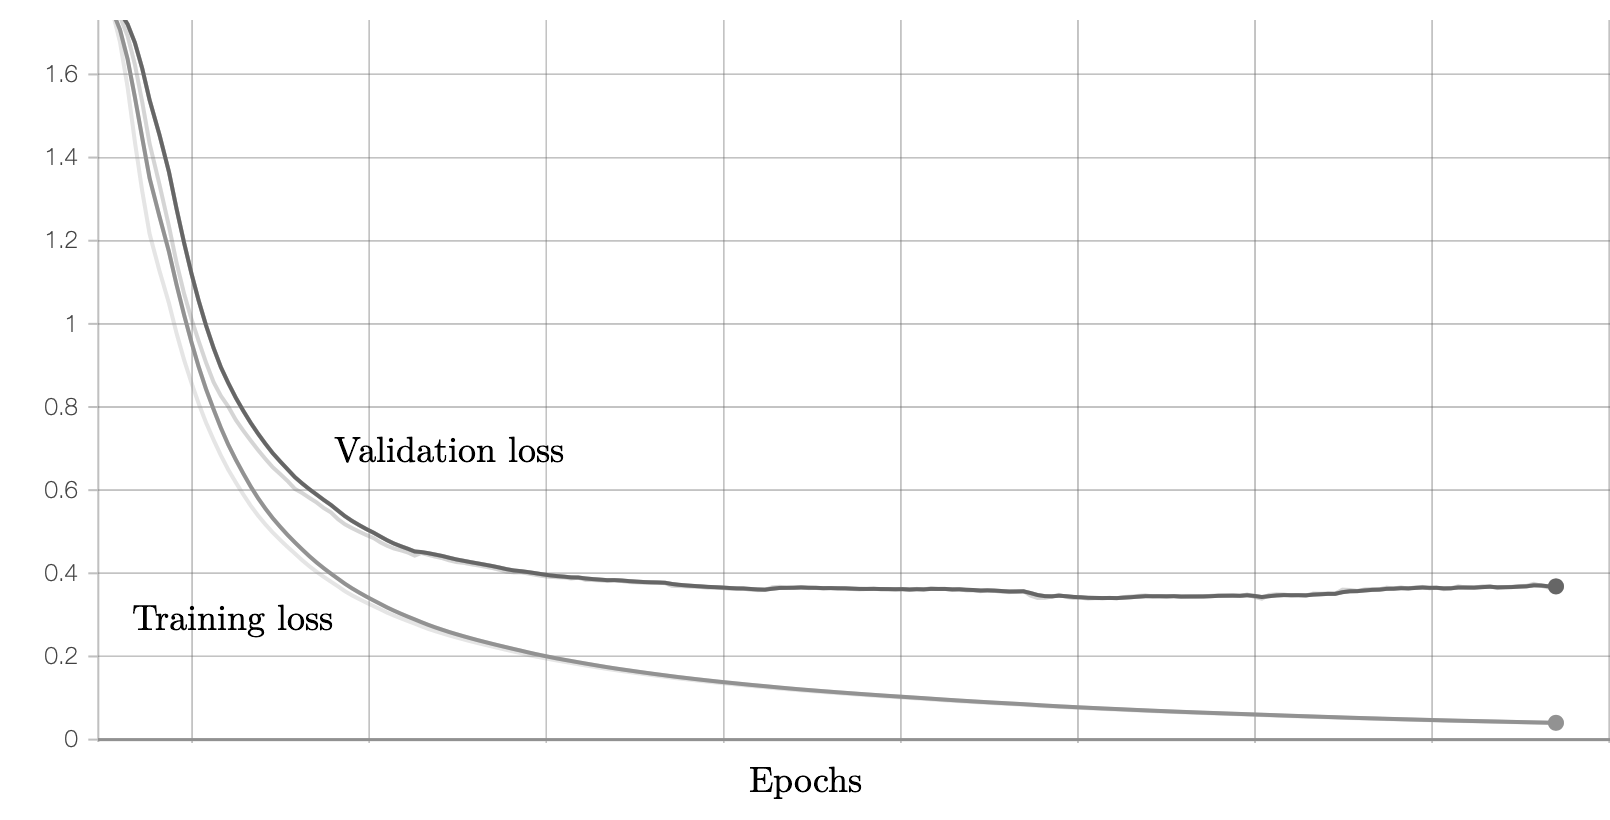
\includegraphics[width=0.65\paperwidth]{img/overfitting.png}}
		\caption{Overfitting due to high kernel size.}
	\end{figure}
\end{center}

\begin{center}
	\begin{figure}[ht]
		\makebox[\textwidth]{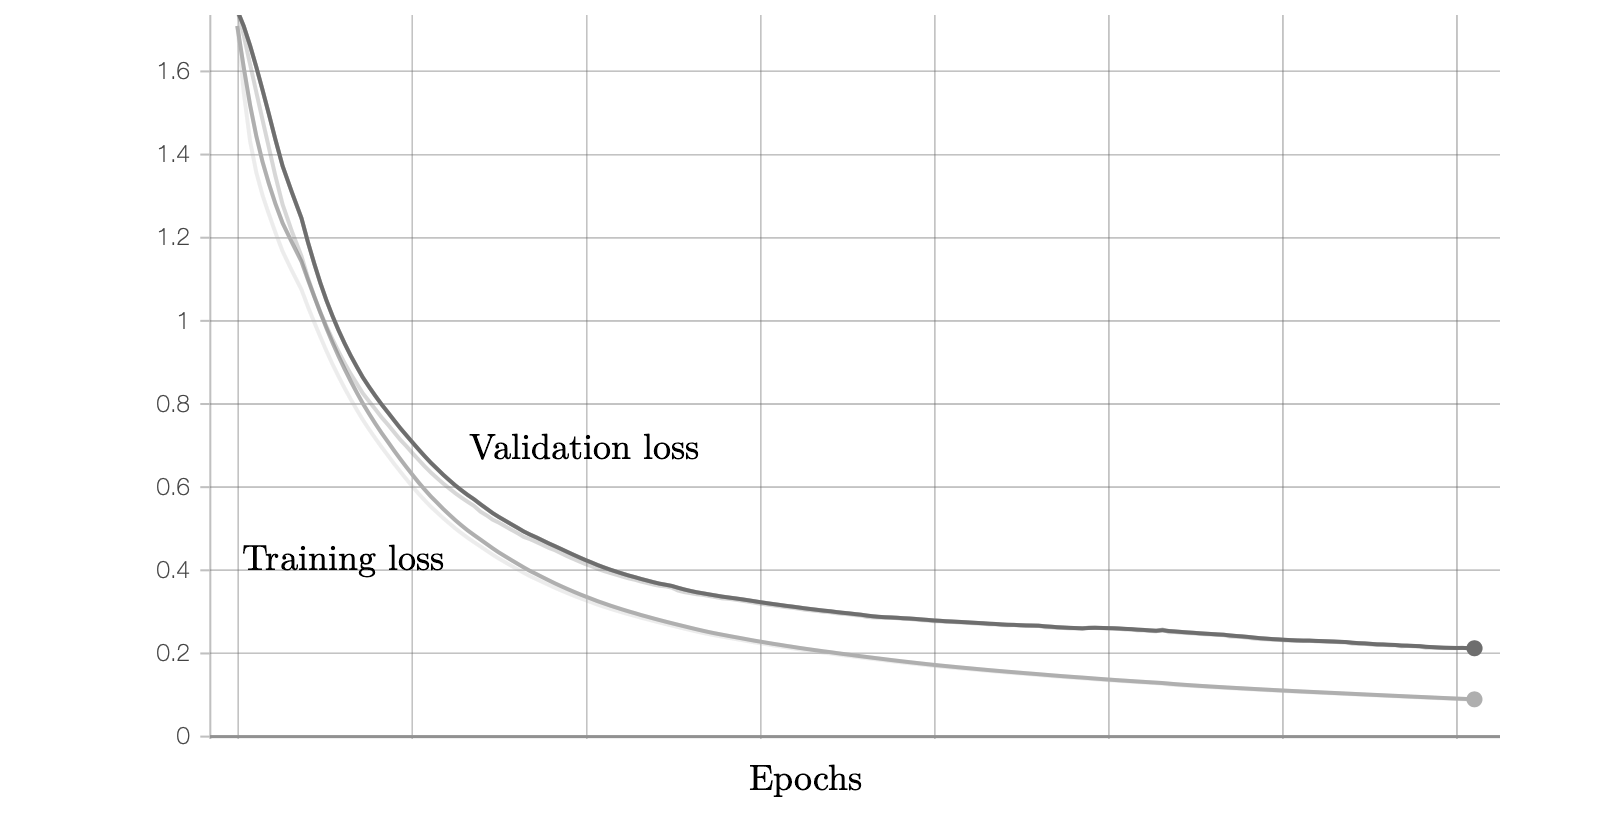
\includegraphics[width=0.65\paperwidth]{img/fitting.png}}
		\caption{Good fitting.}
	\end{figure}
\end{center}

\subsubsection{More accuracy with less data}
The next step was to achieve the maximum accuracy with less possible data. The network was trained several times with different patterns' lengths, and the best choice for a stable and accurate training has proved to be 15 samples per pattern, that with the 22 Hertz sampling means 682 milliseconds long patterns. Up to 11-13 samples, the network was not able to achieve good performance in training, being hard to train and underfitting, while from 17 samples and more, the network fitted the noise, so overfitted.

\begin{center}
	\begin{figure}[ht]
		\makebox[\textwidth]{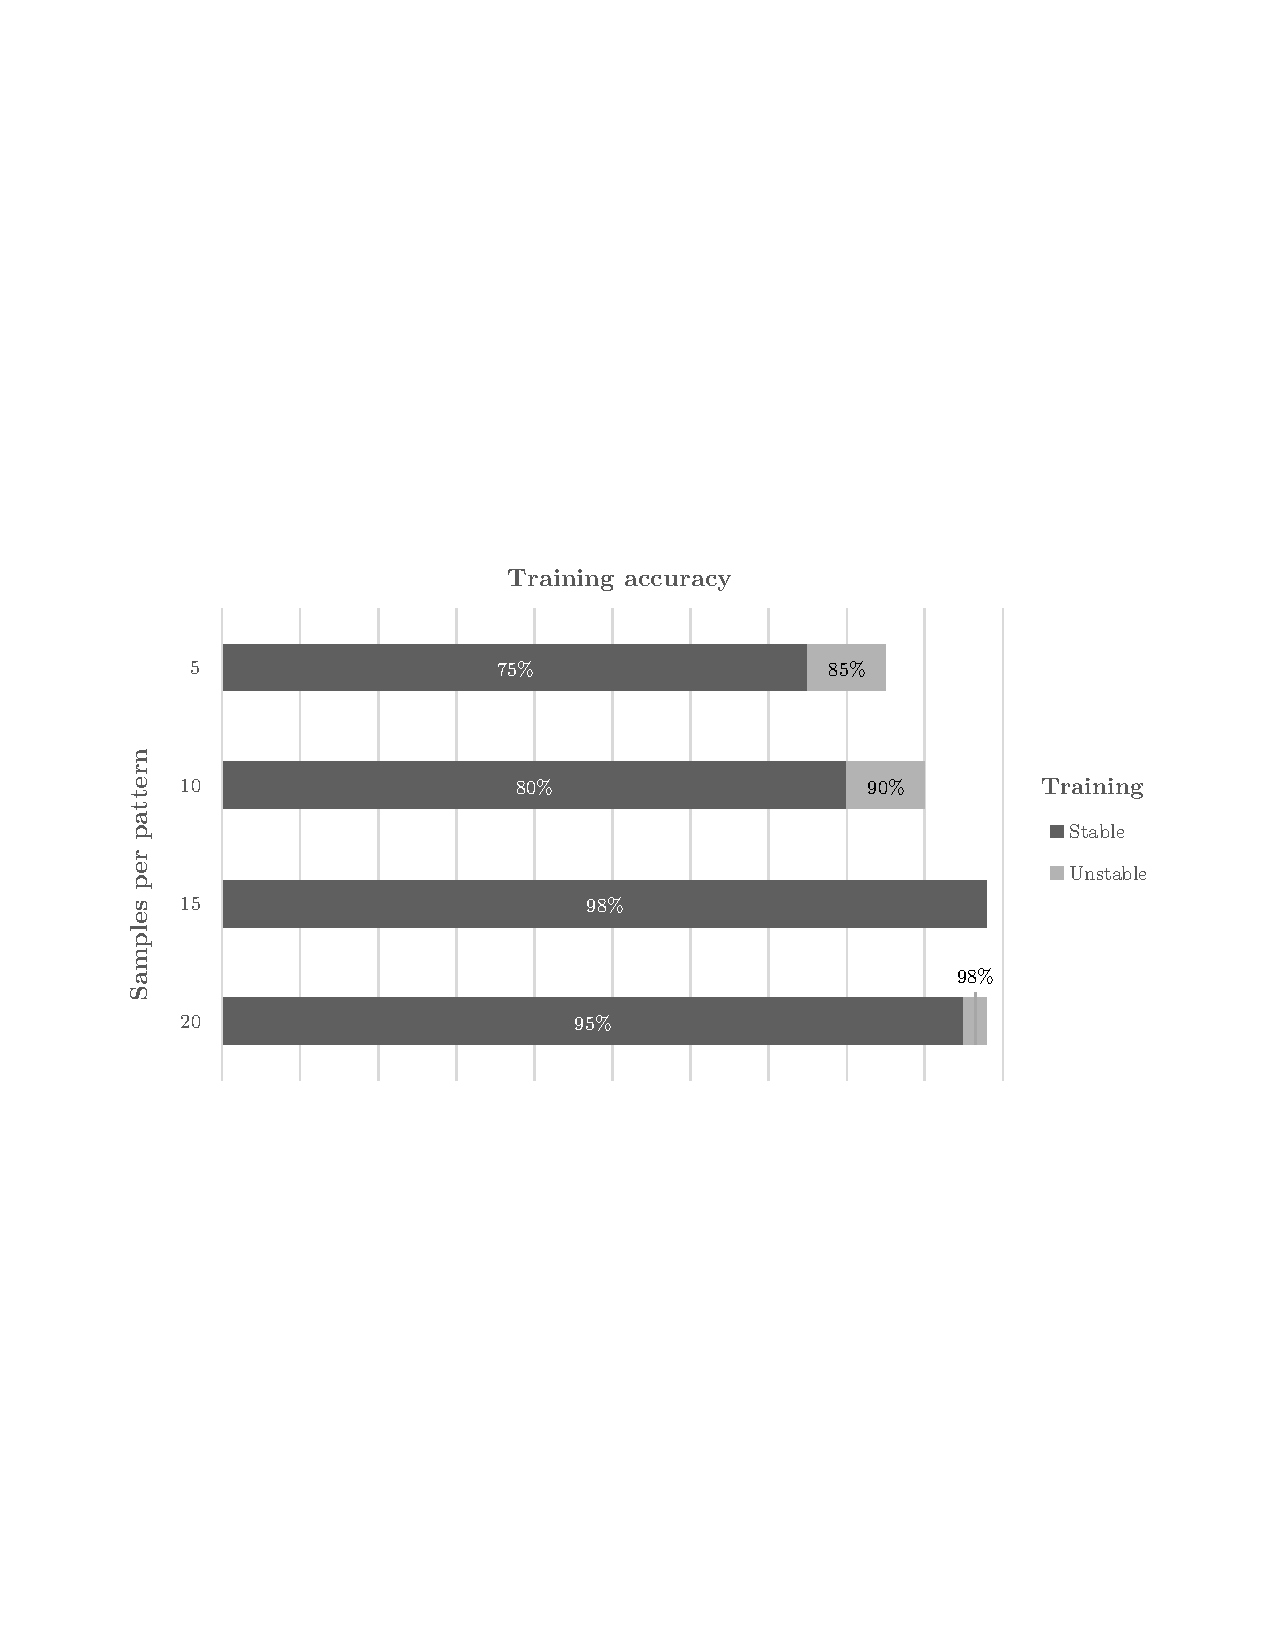
\includegraphics[width=0.65\paperwidth]{img/training_acc_samples.pdf}}
		\caption{Training accuracy with pattern with different lengths.}
	\end{figure}
\end{center}

\subsubsection{Regularization and optimization algorithms}
The convolutional layer's weights are initialized randomly in the uniform range [-0.000001, 0.000001]. To keep under control the network complexity, a \textit{weight decay} approach has been used, with tested values in the range [0.001, 0.05].
\bigbreak

TODO: Why adam optimizer? (paper) Batch size? (useless?)

\subsection{Recurrent neural network}
\subsubsection{Topology, activation functions and hyperparameters}
As done with the TDNN, the input passes through a normalization layer before going to the recurrent layer, and the activation function is \textit{ReLU} for all layers, except for the last one, that uses the \textit{softmax} function, particularly suitable for classification.
\bigbreak

The best topology, that ensured a good fitting without instabilities during the training, is shown in the following schema: one recurrent layer and two densely-connected layers, with two dropout layers before them. In particular, the number of nodes in the recurrent layer was crucial for the model selection:
\begin{itemize}
	\item up to 5 units, the network was able neither to learn the training samples nor generalize;
	\item up to 10 units, the validation accuracy reached almost the 90\%, but then overfitted;
	\item up to 12 units, the network was hard to train, and with 14 units the network was trained smoothly and the validation accuracy grew over 90\%;
	\item from 16 upwards, stricter regularization was needed, but the dropout layers made the training stable and avoided the overfitting. The best number of units was discovered to be 20.
\end{itemize}
The explored range of dropout for both layers was [0, 0.5]. The network was trained with a mini-batch size of 16.

\begin{center}
	\begin{figure}[ht]
		\makebox[\textwidth]{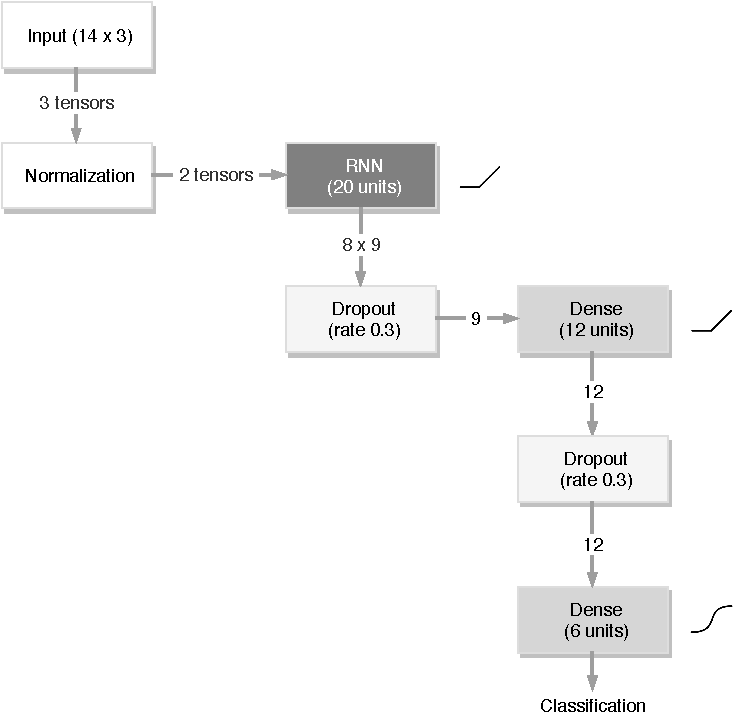
\includegraphics[width=0.55\paperwidth]{img/rnn.pdf}}
		\caption{RNN final topology.}
	\end{figure}
\end{center}

\subsubsection{Features and samples length}
Adding features besides the three acceleration values made the training harder and unstable, even with more layers and more recurrent units. 

In this model, reducing the number of samples has not improved the validation accuracy as for the TDNN, but the performance significantly decreased only for less than 14 samples per pattern, accordingly to the previous results.

\begin{center}
	\begin{figure}[ht]
		\makebox[\textwidth]{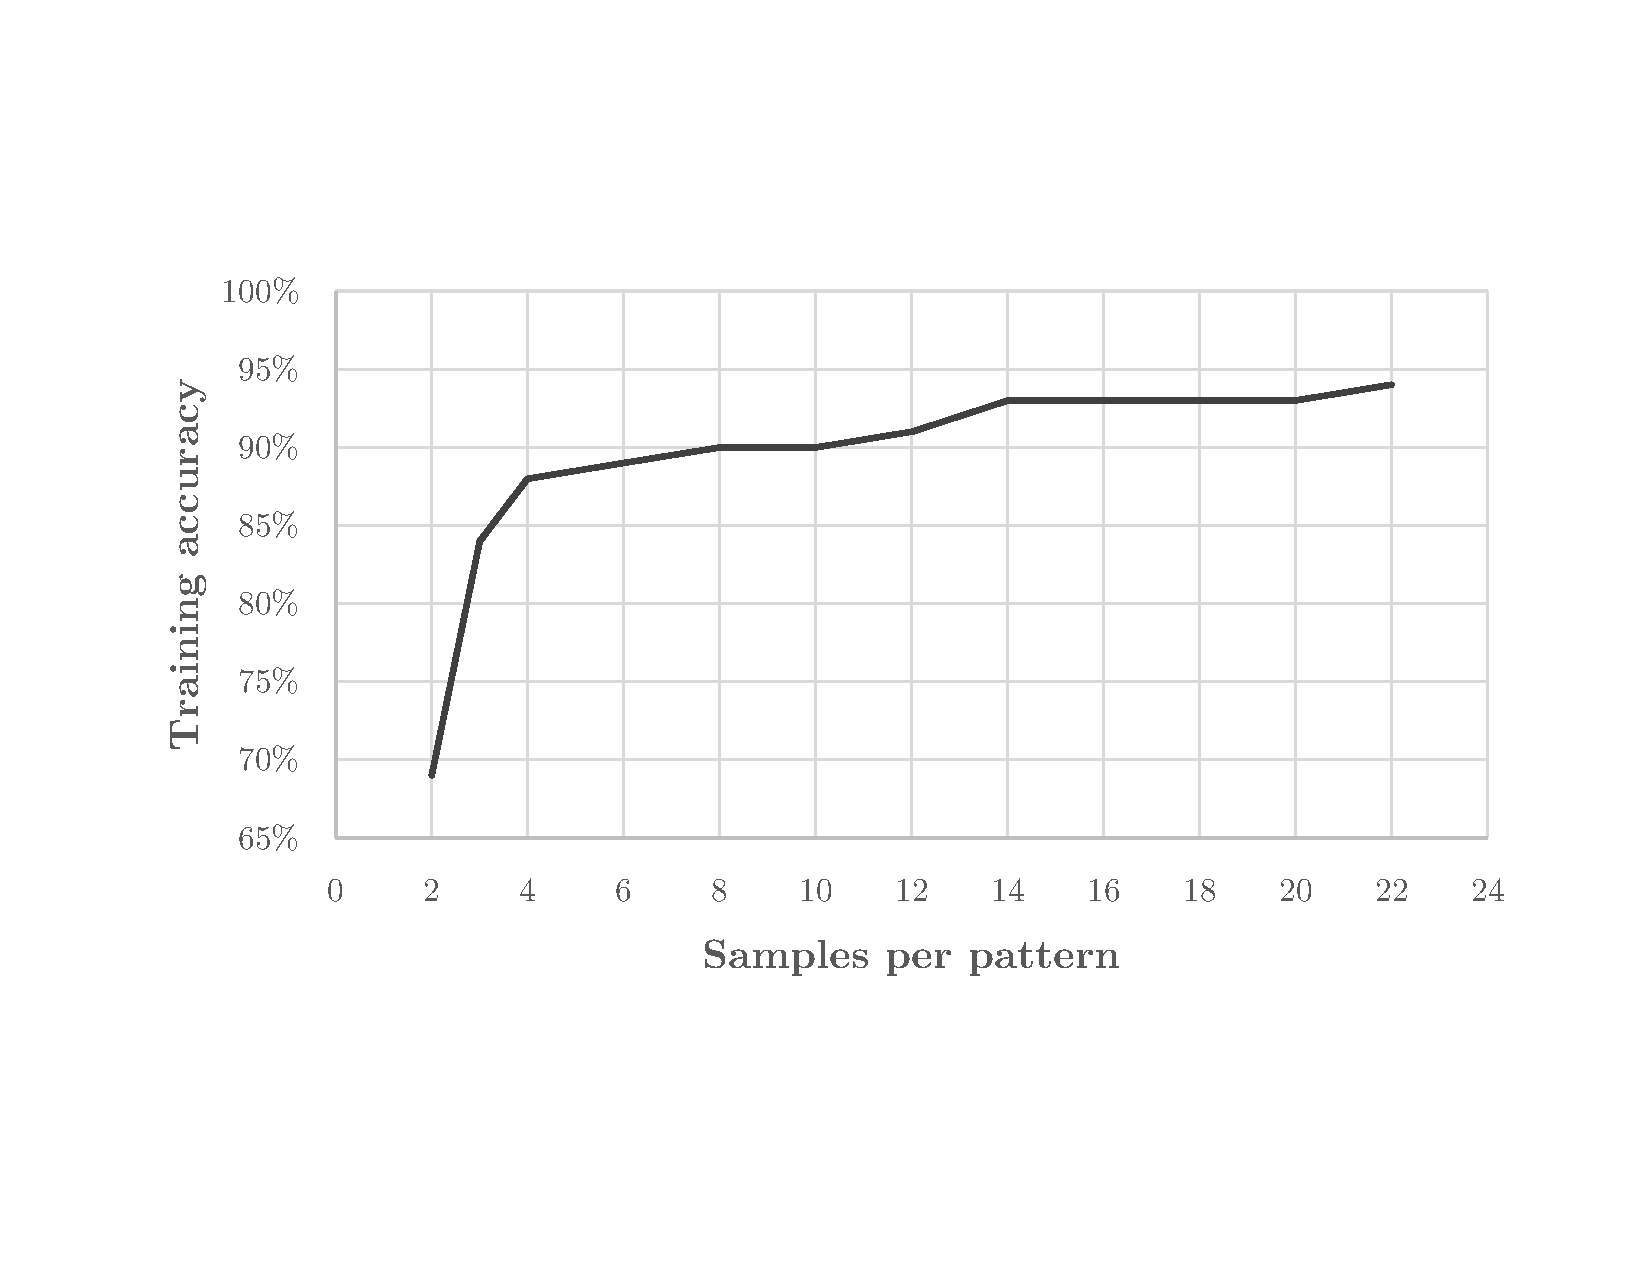
\includegraphics[width=0.6\paperwidth]{img/training_acc_samples_2.pdf}}
		\caption{\dots}
	\end{figure}
\end{center}
